\section{Architecture de l'application}

Dans cette partie je vais m'attarder premièrement sur l'architecture choisie pour faire le lien entre l'interface graphique et la noyau fonctionnel de l'application, puis enfin je décrirai l'architecture adoptée pour implémenter les différents exercices au sein de l'application.

Le diagramme de classes de l'architecture du projet avec les différentes classes qui ont été utilisées est disponible en annexe \ref{appendix:class}.

\subsection{Interface graphique et noyau fonctionnel}
La partie graphique de l'application et la partie fonctionnelle doivent bien entendu être distincte. De plus la partie fonctionnelle doit être indépendante de la partie graphique. Cela permet par exemple de déployer une application web et mobile avec la même partie fonctionnelle, et en définissant simplement 2 interfaces différentes pour le web et le mobile.

L'architecture de l'application est un choix crucial dans le développement d'application. La modification des données de la partie fonctionnelle doit se refléter sur la partie graphique. Un composant graphique dans le monde de Flutter est appelé \textit{widget} (bouton, texte, layout, etc.). La programmation mobile est asynchrone et réactive, des données peuvent être modifiées après un appel réseau, par un utilisateur extérieur ou encore par un autre appareil par exemple ; les widgets doivent réagir à ces changements.

J'ai choisi d'ajouter une couche de providers entre le niveau graphique et le niveau fonctionel. Ces providers fournissent les données necessaires au monde graphique par l'intermédiaire de \textit{stream} (équivalent aux \textit{observable} dans \textit{ReactiveX}). Ici, un stream peut être vu comme un tuyau unidirectionnel, le provider insère des éléments dans ce tuyau, et la partie graphique a accès à la deuxième extremité du tuyau pour accèder à l'élement qu'il y a dans le tuyau. Chaque nouvel élément inséré dans le \textit{stream} remplace l'eventuel ancien élément.

\begin{figure}[H]
  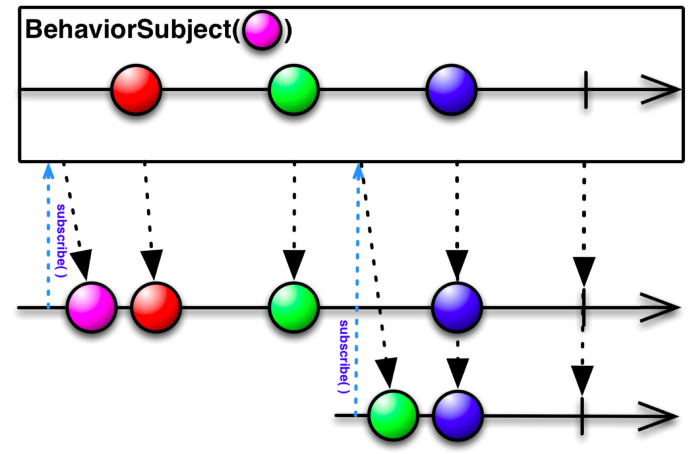
\includegraphics[width=.7\linewidth]{content/imgs/stream.png}
  \caption{\textit{Behaviour subject} comportement}
  \label{fig:stream}
\end{figure}

Il existe le widget \textit{StreamBuilder} qui permet d'écouter la sortie d'un \textit{stream}. Chaque nouvel élément inséré dans le stream a pour effet de reconstruire la descendance de ce widget : tous les fils de ce widget seront réconstruit et redessiner à l'écran. Par exemple, si le champ texte de l'abre de widget de la figure \ref{fig:stream_ex1} dépend d'une donnée de la partie fonctionnelle qui est succeptible de changer au cours du temps et donc qui est disponible via un \textit{stream}, il suffit d'ajouter comme parent à ce widget texte le widget \textit{StreamBuilder} qui va avoir accès à l'extremité du tuyau contenant la donnée à afficher. Ce widget et donc sa descendance (donc le champ texte) se reconstruiront automatiquemet à chaque fois que le contenu du stream change (càd que le provider insère une nouvelle dans le tuyau).

Cette architecture permet de reconstruire seulement les parties de l'interface graphique qui ont \textbf{besoin} d'être reconstruite suite à la modification ou à l'ajout d'une donnée, qui se passe donc du côté fonctionnelle de l'application. C'est une architecture bien plus performante qu'une solution basique qui consisterait à recontruire tout l'arbre de widget à partir de la racine de la page affiché à chaque nouveau changement.

\begin{figure}[H]
  \centering
  \begin{subfigure}{.5\textwidth}
    \centering
    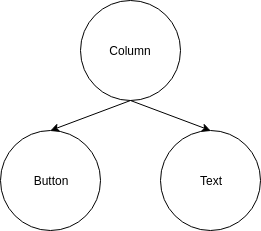
\includegraphics[width=.8\linewidth]{content/imgs/ex1.png}
    \caption{Arbre de widget composé d'un boutton et d'un texte}
    \label{fig:stream_ex1}
  \end{subfigure}%
  \begin{subfigure}{.5\textwidth}
    \centering
    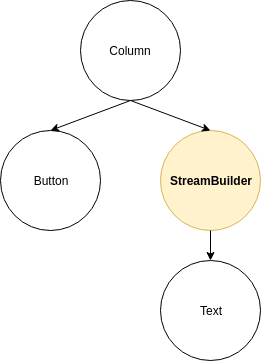
\includegraphics[width=.8\linewidth]{content/imgs/ex2.png}
    \caption{Architecture de l'arbe avec un \textit{StreamBuilder}}
  \end{subfigure}
  \caption{Universiti Teknologi PETRONAS}
\end{figure}

\subsection{Architecture des exercices}

Un aspect de l'application intéressant à concevoir était la structure des exercices. Les exercices sont différents mais partagent tout de même beaucoup de points communs, il était donc nécessaire de trouver une architecture permettant d'implémenter différents exercices rapidement sans re-developper toute la base de l'exercice à chaque fois.

\begin{figure}[H]
  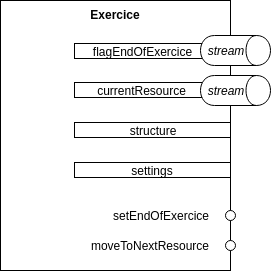
\includegraphics[width=150px]{content/imgs/exercice.png}
  \caption{Structure d'un exercice}
  \label{fig:exercice}
\end{figure}

L'architecture choisie est la suivante : un exercice possède simplement les attributs suivants :

\begin{itemize}
  \item Une \textbf{strucutre} : la liste des éléments constituant l'exercice. Plusieurs éléments peuvent être utilisés par un exercice, par exemple : un enregistreur vocal, un afficheur de mot, phrase ou texte, un metronome, etc. ;
  \item Des \textbf{réglages} : les réglages de l'exercice (choisis par l'utilisateur ou directement imposé par l'exercice). Ces réglages sont identifiés par un identifiant unique et associé à une valeur (booléen, entier, etc.) ;
  \item La \textbf{resource courrante} : la resource actuellement utilisée par l'exercice (mot, phrase, texte) ;
  \item Un \textbf{flag} pour signaler la fin de l'exercice.
\end{itemize}

\textit{Note : pour faire simple j'ai omis certaines informations comme la date de création, l'intitulé, etc).}

\paragraph{Structure}
Comme vu précedemment, la structure d'un exercice est consituée de plusieurs éléments (concrétement ces éléments sont les valeurs d'un type énuméré). Côté graphique, il y a un convertisseur de ces valeurs en un oject graphique. Par exemple l'élément \textit{metronome} sera associé à un widget qui affiche un métronome avec un signal visuel et un signal sonor à tempo régulier. Ces objets graphiques ont accès aux attributs et à certaines méthodes de l'exercice. Par exemple le widget permettant d'afficher une resource (mot, phrase, texte), a accès à la resource courante de l'exercice et peux appeler la fonction \texttt{moveToNextResource} pour changer la resource courante. Ces widgets peuvent aussi accéder aux réglages de l'exercices.

\begin{figure}[H]
  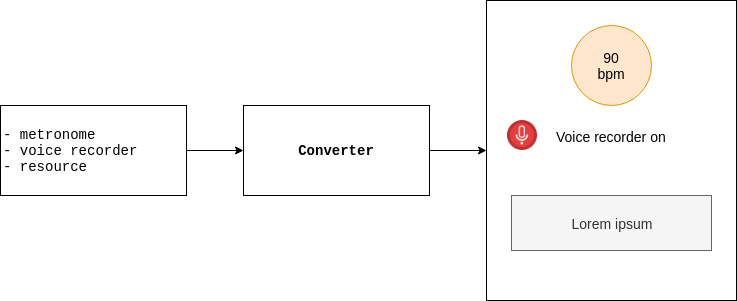
\includegraphics[width=0.8\linewidth]{content/imgs/struc.png}
  \caption{De la structure à l'interface}
  \label{fig:struc}
\end{figure}

\paragraph{Réglages}
Chaque exercice peut définir sa liste de réglages. Ces réglages sont destinés à être utilisé par les \textit{widgets} associés aux éléments de la structure des exercices. Par exemple l'exerice du métronome peut définir un réglages \texttt{metronome\_bpm} qui va permettre au widget affichant le métronome de régler la valeur du tempo suivant ce réglage. Comme pour les élements de la structure des exercices, il y a un convertisseur des réglages en un object graphique permettant de modifier ces réglages.

\begin{figure}[H]
  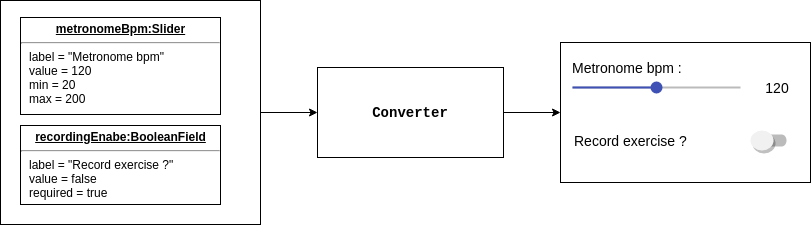
\includegraphics[width=0.8\linewidth]{content/imgs/settings.png}
  \caption{Génération visuelle des réglages de l'exercice}
  \label{fig:settings}
\end{figure}

Cette architecture permet de construire facilement et rapidement un large panel d'exercices. Pour structurer un nouvel exercice il suffit de piocher dans la collection déjà existante si tous les éléments nécessaires à l'élaboration de l'exercice y sont disponible. Dans le cas échéant, il suffit juste de developper l'élément manquant.






% eof
